\section{Test cases for simple statecharts}
\label{testSimpeState}

For this section, we consider only statecharts that do not contain hierarchy and concurrency. Statecharts with hierarchy and concurrency will be explained later.


We start by making sure every reachable state in the statechart is covered. In order to do so, for each state $s$ in the statechart, we construct a path $p$ from the initial state to $s$. The path $p$ in said to be the coverage path of $s$. All coverage paths generated are stored in a set called \textit{State Cover}, which is denoted by $C$. Therefore, $C$ is a set of sequence of transition labels, such that we can find an element from this set to reach any desired state starting from the initial one \cite{bogdanov}.

Since there is no hierarchy or concurrency in the statechart, the construction of $C$ is similar to covering states of an automaton and it can be done through a depth search in the states. Find below a pseudocode for the method:

\begin{lstlisting}
//Wrap method to contrusct the State Cover
//It receives as argument the initial state of the statechart
Set constructSetC(State initialState) {
	
	Set setC = new Set();

	Path emptyPath = "";

	List visited = new List();

	return constructSetCRec(initalState,emptyPath,setC);
}
\end{lstlisting}


\begin{lstlisting}
//Recursive function that will do all the work
//returns the State Cover set, or set C
Set constructSetCRec(State s, Path p, Set setC, List visited) {

	visited.add(s);

	setC.add(s,p);
	
	for (Transition t in s.getOutgGoingTransitions()) {
		
		State nextState = t.getDestiny();

		if (!visited.contains(nextState)) {

			Path nextCoveragePath = p + t.getLabel());

			constructSetCRec(nextState,nextCoveragePath,setC,visited);		
		}
	}
	
	return setC;
}

\end{lstlisting}

Now that we have the coverage for every reachable state, we need to trigger each transition on each state and create the test cases. For each transition there will be a test case, thus every transition in the diagram will be exercides at least once during testing.

Consider the transition $t = (s,l,q)$, where $s$ is the original state, $l$ is the event label that triggers $t$ and $q$ is the destiny state. Previously, we computed that $s$ has coverage path $p$ such that $p \in C$ and $p$ is a sequence of label. The test case $TC$ to $t$ would be the concatenation of the event label $l$ to the end of $p$ expecting to get to state $q$. The process is repeated to every transition in the statechart. Find below the algorithm for the test case creation:

\begin{lstlisting}[label={pseudocodeTestCase}]
//Function that prints the test cases for all transitions in a statechart
void generateTestCases(Statechart sc, Set setC) {

	for (State s in sc.getStates()) {
	
		print("At state "+s.getName());

		Path coveragePath = setC.getCoveragePath(s);

		for (Transition t in s.getOutgGoingTransitions()) {

			print("Test case for "+t.getLabel());

			Path testPath = coveragePath + t.getLabel();

			print("Test path: "+testPath);

			State expectedState = t.getDestiny();

			print("Expected state: "+expectedState);
		}
	}
}
\end{lstlisting}


Consider the following example in figure \ref{fig:trocaPlano} where we model the verifications in a purchase flow of a telco ecommerce. The flow is done by a user who wishes to change their cellphone plan. They will be able to change plan if their not employees from the telco company and are not committed to a loyalty contract.

\begin{figure}[htb]
\centering
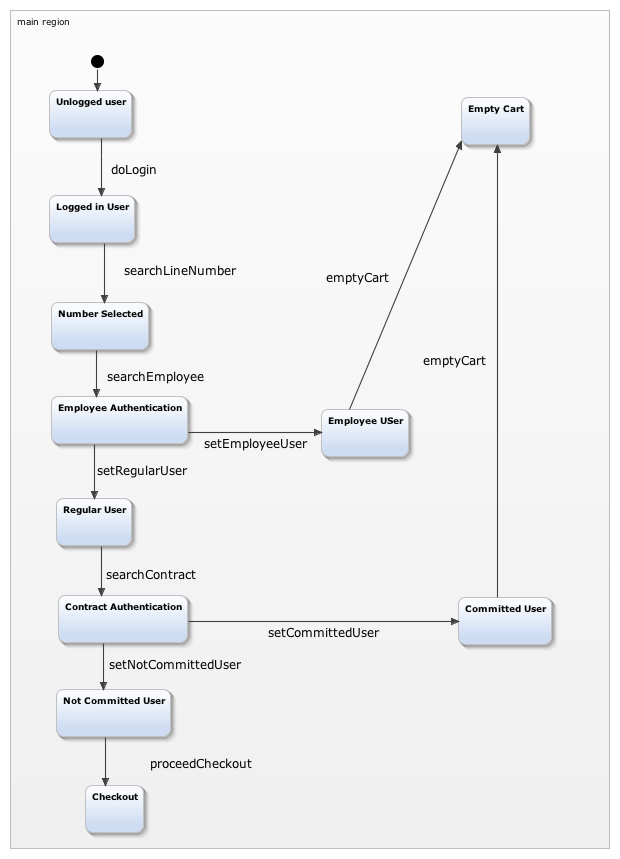
\includegraphics[width=10cm]{figuras/trocaPlano}
\caption{\label{fig:trocaPlano} A plan change flow statechart in a telco ecommerce}
\end{figure}

Hierarchy and orthogonality are not found in statechart \ref{fig:trocaPlano}. Hence, we can apply the the technique just presented.

The construction of the \textit{State Cover} set, or $C$, goes as follows:

We start at the inital state \textit{Unlogged User}. Since it is the initial state, its coverage path is the emtpy string, denoted by $e$.

Next, we recursively visit the states that can be reached from \textit{Unlogged User}. In our example, we get to state \textit{Logged in User}. In order to get to this state, it was necessary to go through transition $doLogin$. Therefore, the coverage path for \textit{Logged in User} is \textit{e doLogin}. Note that we concatenate the coverage path of the previous state to the transition taken.

When construction of $C$ is done, we have the following covage paths:

\begin{center}
\begin{tabular}{| l | p{10cm}|}

\hline

State & Coverage path \\ \hline

Unlogged user & e \\ \hline

Logged in User & e doLogin\\ \hline 

Number Selected & e doLogin searchLineNumber\\ \hline

Employee Authentication & e doLogin searchLineNumber searchEmployee\\ \hline

Employee User & e doLogin searchLineNumber searchEmployee setEmployeeUser \\ \hline

Empty Cart & e doLogin searchLineNumber searchEmployee setEmployeeUser emptyCart \\ \hline

Regular User & doLogin searchLineNumber searchEmployee setRegularUser \\ \hline

Contract Authentication & doLogin searchLineNumber searchEmployee setRegularUser searchContract \\ \hline

Committed User & doLogin searchLineNumber searchEmployee setRegularUser searchContract setCommittedUser \\ \hline

Not Committed User & doLogin searchLineNumber searchEmployee setRegularUser searchContract setNotCommittedUser \\ \hline

Checkout & doLogin searchLineNumber searchEmployee setRegularUser searchContract setNotCommittedUser proceedCheckout\\
\hline
\end{tabular}
\end{center}

Notice the empty string $e$ is present due to the unlabeled transition leaving the initial state.

Then, we have to create a test case for every transition leaving each state. Let's take state \textit{Employee Authentication} for example. It has two leaving transitions: $setEmployeeUser$ and $setRegularUser$. To guarantee they are exercided at least once during testing and that they go to their appropriate destiny states, we need the following test cases:

\begin{itemize}

\item Test case for \textit{\textbf{setEmployeeUser}}

Path: \textit{e doLogin searchLineNumber searchEmployee setEmployeeUser}

Expected state: \textit{Employee User}

\item Test case for \textit{\textbf{setRegularUser}}

Path: \textit{e doLogin searchLineNumber searchEmployee setRegularUser}

Expected state: \textit{Regular User}
\end{itemize}

Note that the path to test is the coverage page of the origin state concatenated with the label of the tested transition. The analogous is done for all other transitions in the model.

